% =====================================================================
%  Ofrenda Viva — Speech de presentación de producto (Día de Muertos)
%  iOS Development Lab · Compila con pdfLaTeX (Overleaf), XeLaTeX o LuaLaTeX
% =====================================================================
\documentclass[aspectratio=169,11pt]{beamer}
\usepackage{comment}

\usepackage{iftex}
\ifPDFTeX
  % pdfLaTeX (por defecto en Overleaf)
  \usepackage[utf8]{inputenc}
  \usepackage[T1]{fontenc}
  \IfFileExists{tgheros.sty}{\usepackage{tgheros}}{\usepackage[scaled]{helvet}}
  \usepackage{textcomp}
\else
  % XeLaTeX / LuaLaTeX
  \usepackage{fontspec}
  \setsansfont{TeX Gyre Heros}
\fi
\usepackage{tikz}
\usepackage{multimedia} % video en el PDF (se reproduce en Adobe Acrobat Reader)
\usetikzlibrary{positioning,shapes,arrows.meta,calc,shadows}

% ---------- Paleta Día de Muertos ----------
\definecolor{noche}{HTML}{2B1740}      % morado noche
\definecolor{nochesuave}{HTML}{3E2459}
\definecolor{cempa}{HTML}{F28C1B}      % cempasúchil
\definecolor{rosa}{HTML}{E0457B}       % rosa mexicano
\definecolor{vela}{HTML}{FFD166}       % luz de vela
\definecolor{papel}{HTML}{FFF6EC}      % fondo claro
\definecolor{tinta}{HTML}{2E2433}
\definecolor{gris}{HTML}{8A7F90}

% ---------- Tema propio ----------
\setbeamertemplate{navigation symbols}{}
\setbeamercolor{background canvas}{bg=papel}
\setbeamercolor{normal text}{fg=tinta}
\setbeamercolor{frametitle}{fg=noche}
\setbeamercolor{structure}{fg=rosa}
\setbeamercolor{alerted text}{fg=rosa}
\setbeamerfont{frametitle}{size=\Large,series=\bfseries}
\setbeamertemplate{itemize item}{\color{cempa}\large$\bullet$}
\setbeamertemplate{itemize subitem}{\color{rosa}$\circ$}
\setbeamertemplate{enumerate item}{\color{cempa}\bfseries\insertenumlabel.}

% Barra superior: papel picado
\newcommand{\papelpicado}{%
  \begin{tikzpicture}[remember picture,overlay]
    \foreach \i/\c in {0/cempa,1/rosa,2/vela,3/nochesuave,4/cempa,5/rosa,6/vela,7/nochesuave,8/cempa,9/rosa,10/vela,11/nochesuave,12/cempa,13/rosa,14/vela,15/nochesuave}{
      \fill[\c] ($(current page.north west)+(\i*1.0,0)$) -- ++(1.0,0) -- ++(0,-0.30)
        -- ++(-0.25,-0.12) -- ++(-0.25,0.12) -- ++(-0.25,-0.12) -- ++(-0.25,0.12) -- cycle;
    }
  \end{tikzpicture}}

\makeatletter
\setbeamertemplate{frametitle}{%
  \papelpicado
  \begin{tikzpicture}[remember picture,overlay]
    \node[anchor=north west,inner sep=0,align=left] at ($(current page.north west)+(0.55,-0.6)$) {%
      \usebeamerfont{frametitle}\usebeamercolor[fg]{frametitle}\insertframetitle
      \ifx\beamer@framesubtitle\@empty\else\\[2pt]{\normalfont\normalsize\color{gris}\insertframesubtitle}\fi\\[-2pt]
      {\color{cempa}\rule{2.2cm}{2pt}}};
  \end{tikzpicture}%
  \vspace*{\ifx\beamer@framesubtitle\@empty 1.0cm\else 1.5cm\fi}}
\makeatother

\setbeamertemplate{footline}{%
  \hfill{\scriptsize\color{gris}Ofrenda Viva \quad\insertframenumber\,/\,\inserttotalframenumber}\hspace*{0.5cm}\vspace*{0.25cm}}

% Etiqueta de quién habla
\newcommand{\habla}[1]{%
  \begin{tikzpicture}[remember picture,overlay]
    \node[anchor=north east,fill=noche,text=vela,rounded corners=6pt,font=\scriptsize\bfseries,inner sep=4pt]
      at ($(current page.north east)+(-0.4,-0.55)$) {Habla: #1};
  \end{tikzpicture}}

% Tarjeta de contenido
\newcommand{\tarjeta}[3]{% color, título, texto
  \begin{tikzpicture}[baseline=(current bounding box.north)]
    \node[fill=white,draw=#1,line width=1.2pt,rounded corners=8pt,text width=3.7cm,minimum height=2.4cm,align=left,inner sep=8pt,drop shadow={opacity=0.15}] {%
      \raggedright\hyphenpenalty=10000{\color{#1}\bfseries #2}\\[4pt]\small #3};
  \end{tikzpicture}}

% ---------- Mockup de iPhone ----------
% \iphone{posición}{título pantalla}{contenido tikz (coordenadas relativas a (0,0)=esquina sup. izq. de la pantalla)}
\newcommand{\iphone}[3]{%
  \begin{scope}[shift={#1}]
    \fill[black!85,rounded corners=14pt,drop shadow={opacity=0.25}] (-0.15,0.15) rectangle (3.35,-6.55);
    \fill[papel,rounded corners=10pt] (0,0) rectangle (3.2,-6.4);
    \fill[black!85,rounded corners=3pt] (1.15,-0.12) rectangle (2.05,-0.32); % dynamic island
    \node[anchor=north,font=\scriptsize\bfseries,text=noche] at (1.6,-0.45) {#2};
    \draw[gris!40] (0.15,-0.82) -- (3.05,-0.82);
    #3
    % tab bar
    \fill[white] (0.02,-5.85) rectangle (3.18,-6.25);
    \foreach \x/\l in {0.45/Inicio,1.15/Familia,1.95/Ofrenda,2.75/Perfil}{
      \fill[gris!60] (\x,-5.95) circle (0.07);
      \node[font=\fontsize{4}{4}\selectfont,text=gris] at (\x,-6.12) {\l};}
  \end{scope}}

\tikzset{per/.style={circle,fill=#1,minimum size=0.55cm,inner sep=0,font=\fontsize{4}{4}\selectfont\bfseries,text=white}}

\tikzset{paso/.style={fill=white,draw=#1,line width=1.4pt,rounded corners=8pt,text width=2.5cm,minimum height=2.6cm,align=center,font=\small,inner ysep=12pt},
  num/.style={circle,fill=#1,text=white,font=\bfseries,minimum size=0.6cm},
  flecha/.style={-{Stealth[length=3mm]},line width=1.5pt,color=gris}}

\title{Ofrenda Viva}
\subtitle{Que nadie en la ofrenda sea un desconocido}
\author{Integrante 1 \and Integrante 2 \and Integrante 3}
\institute{iOS Development Lab · Servicio Social}
\date{30 de octubre de 2026}

\hyphenpenalty=10000\exhyphenpenalty=10000
% Separador de sección
\newcommand{\seccion}[3]{% número, nombre, frase
{\setbeamercolor{background canvas}{bg=noche}
\begin{frame}[plain]
  \papelpicado
  \vspace{1.5cm}
  {\color{cempa}\fontsize{54}{54}\selectfont\bfseries #1}\\[6pt]
  {\color{white}\fontsize{30}{34}\selectfont\bfseries #2}\\[10pt]
  {\color{vela}\large #3}
\end{frame}}}

% Diapositiva oscura de una sola idea
\newcommand{\declaracion}[1]{%
{\setbeamercolor{background canvas}{bg=noche}
\begin{frame}[plain]
  \papelpicado
  \vfill
  \begin{center}#1\end{center}
  \vfill
\end{frame}}}

% Icono en círculo
\newcommand{\icono}[2]{% color, dibujo
  \begin{tikzpicture}
    \fill[#1] (0,0) circle (0.9);
    #2
  \end{tikzpicture}}

\newcommand{\pInicio}{%
    \iphone{(0,0)}{Ofrenda Viva}{
      \node[anchor=west,font=\fontsize{6}{7}\selectfont\bfseries,text=noche] at (0.2,-1.1) {Familia Hernández};
      \node[anchor=west,font=\fontsize{4.5}{5}\selectfont,text=gris] at (0.2,-1.35) {12 seres queridos · 8 familiares};
      \fill[cempa,rounded corners=5pt] (0.2,-1.6) rectangle (3.0,-2.55);
      \node[text=white,font=\fontsize{5}{6}\selectfont\bfseries,align=left,anchor=west] at (0.3,-2.07) {Faltan 3 días para\\Día de Muertos};
      \node[anchor=west,font=\fontsize{5.5}{6}\selectfont\bfseries,text=noche] at (0.2,-2.85) {Recuerdo del día};
      \fill[white,rounded corners=4pt] (0.2,-3.05) rectangle (3.0,-4.15);
      \fill[gris!30,rounded corners=3pt] (0.3,-3.15) rectangle (1.1,-4.05);
      \node[anchor=north west,text width=1.7cm,font=\fontsize{4.5}{5.5}\selectfont,text=tinta] at (1.15,-3.15) {\textbf{Bisabuela Rosa} hacía el mejor mole de todo el pueblo.};
      \node[anchor=west,font=\fontsize{5.5}{6}\selectfont\bfseries,text=noche] at (0.2,-4.45) {Actividad reciente};
      \foreach \y/\t in {-4.75/Tía Lupe subió 3 fotos,-5.15/Abuelo grabó un audio}{
        \fill[rosa] (0.3,\y) circle (0.08);
        \node[anchor=west,font=\fontsize{4.5}{5}\selectfont,text=tinta] at (0.45,\y) {\t};}
    }}
\newcommand{\pPerfil}{%
    \iphone{(0,0)}{Perfil}{
      \fill[gris!30] (1.6,-1.65) circle (0.6);
      \node[font=\fontsize{4.5}{5}\selectfont,text=gris] at (1.6,-1.65) {foto};
      \node[font=\fontsize{6.5}{7}\selectfont\bfseries,text=noche] at (1.6,-2.45) {José Hernández};
      \node[font=\fontsize{4.5}{5}\selectfont,text=gris] at (1.6,-2.7) {1932 – 2004 · Tu bisabuelo};
      \node[font=\fontsize{4.5}{5}\selectfont,text=gris] at (1.6,-2.9) {Nació en Oaxaca};
      \foreach \x/\t/\c in {0.25/Historia/rosa,1.2/Fotos/white,2.15/Audios/white}{
        \fill[\c,rounded corners=3pt,draw=rosa] (\x,-3.1) rectangle ++(0.85,-0.3);
        \node[font=\fontsize{4.5}{5}\selectfont] at (\x+0.425,-3.25) {\t};}
      \node[anchor=north west,text width=2.6cm,font=\fontsize{4.5}{5.5}\selectfont,text=tinta] at (0.2,-3.55)
        {Era carpintero. Le encantaba cantar boleros y siempre traía dulces de tamarindo en la bolsa para sus nietos\ldots};
      \fill[white,rounded corners=4pt] (0.2,-4.65) rectangle (3.0,-5.6);
      \node[anchor=west,font=\fontsize{4.5}{5}\selectfont\bfseries,text=noche] at (0.3,-4.85) {Para su ofrenda};
      \node[anchor=west,font=\fontsize{4.5}{5}\selectfont,text=tinta] at (0.3,-5.1) {Tamales · Café de olla};
      \node[anchor=west,font=\fontsize{4.5}{5}\selectfont,text=tinta] at (0.3,-5.35) {Pan dulce · Boleros};
    }}
\newcommand{\pRecuerdos}{%
    \iphone{(0,0)}{Recuerdos de José}{
      \foreach \y/\autor/\t in {-1.05/Abuela Carmen/Nos llevaba al río los domingos,-2.25/Tío Beto/Me enseñó a usar el serrucho}{
        \fill[white,rounded corners=4pt] (0.2,\y) rectangle (3.0,\y-1.05);
        \fill[cempa] (0.4,\y-0.25) circle (0.12);
        \node[anchor=west,font=\fontsize{4.5}{5}\selectfont\bfseries,text=noche] at (0.6,\y-0.25) {\autor};
        \node[anchor=north west,text width=2.5cm,font=\fontsize{4.5}{5.5}\selectfont,text=tinta] at (0.3,\y-0.45) {\t};}
      % nota de voz
      \fill[noche,rounded corners=4pt] (0.2,-3.45) rectangle (3.0,-4.1);
      \fill[vela] (0.5,-3.775) circle (0.15);
      \fill[noche] (0.45,-3.69) -- (0.45,-3.86) -- (0.6,-3.775) -- cycle;
      \foreach \x/\h in {0.8/0.1,0.9/0.2,1.0/0.15,1.1/0.25,1.2/0.1,1.3/0.2,1.4/0.28,1.5/0.12,1.6/0.22,1.7/0.1,1.8/0.18,1.9/0.25,2.0/0.12,2.1/0.2}{
        \draw[vela,line width=1pt] (\x,-3.775+\h/2) -- (\x,-3.775-\h/2);}
      \node[font=\fontsize{4}{5}\selectfont,text=white] at (2.6,-3.775) {1:24};
      \node[anchor=west,font=\fontsize{4}{5}\selectfont,text=gris] at (0.2,-4.25) {Audio de la Abuela Carmen};
      % botón
      \fill[rosa,rounded corners=8pt] (0.5,-4.75) rectangle (2.7,-5.25);
      \node[text=white,font=\fontsize{5}{6}\selectfont\bfseries] at (1.6,-5.0) {+ Agregar recuerdo};
    }}
\newcommand{\pArbol}{%
    \iphone{(0,0)}{Árbol familiar}{
      \node[per=gris] (j) at (1.1,-1.4) {José};
      \node[per=gris] (r) at (2.1,-1.4) {Rosa};
      \node[per=cempa] (c) at (1.6,-2.6) {Carmen};
      \node[per=gris] (p) at (0.6,-2.6) {Pedro};
      \node[per=rosa] (m) at (1.1,-3.8) {Mamá};
      \node[per=rosa] (b) at (2.3,-3.8) {Beto};
      \node[per=noche] (t) at (1.1,-5.0) {Tú};
      \draw[gris] (j) -- (r); \draw[gris] (1.6,-1.4) -- (c);
      \draw[gris] (p) -- (c); \draw[gris] (1.1,-2.6) -- (m); \draw[gris] (1.1,-2.6) -- (1.7,-3.2) -- (b);
      \draw[gris] (m) -- (t);
      \node[font=\fontsize{4}{4}\selectfont,text=gris,anchor=west] at (2.0,-5.0) {gris = fallecido};
    }}
\newcommand{\pOfrenda}{%
    \iphone{(0,0)}{Mi ofrenda}{
      \fill[noche,rounded corners=4pt] (0.2,-1.0) rectangle (3.0,-5.6);
      % niveles
      \fill[rosa!80] (0.45,-1.8) rectangle (2.75,-2.0);
      \fill[rosa!65] (0.35,-3.05) rectangle (2.85,-3.25);
      \fill[rosa!50] (0.25,-4.3) rectangle (2.95,-4.5);
      % fotos
      \foreach \x in {0.8,1.6,2.4}{\fill[papel] (\x-0.25,-1.2) rectangle (\x+0.25,-1.75);
        \fill[gris!40] (\x-0.2,-1.25) rectangle (\x+0.2,-1.6);}
      % velas
      \foreach \x in {0.6,1.6,2.6}{\fill[papel] (\x-0.06,-2.6) rectangle (\x+0.06,-3.0);
        \fill[vela] (\x,-2.5) ellipse (0.05 and 0.1);}
      % flores
      \foreach \x in {0.5,0.9,1.3,1.9,2.3,2.7}{\fill[cempa] (\x,-4.15) circle (0.1);}
      \node[font=\fontsize{4}{5}\selectfont,text=white] at (1.6,-3.6) {pan · agua · sal · mole};
      \node[font=\fontsize{4}{5}\selectfont,text=vela,align=center] at (1.6,-5.0) {Toca un elemento para\\conocer su significado};
    }}
\newcommand{\pQR}{%
    \iphone{(0,0)}{Escanear foto}{
      \fill[black!80,rounded corners=4pt] (0.2,-1.0) rectangle (3.0,-4.3);
      \draw[vela,line width=1.5pt] (0.7,-1.5) -- (0.7,-1.8); \draw[vela,line width=1.5pt] (0.7,-1.5) -- (1.0,-1.5);
      \draw[vela,line width=1.5pt] (2.5,-1.5) -- (2.5,-1.8); \draw[vela,line width=1.5pt] (2.5,-1.5) -- (2.2,-1.5);
      \draw[vela,line width=1.5pt] (0.7,-3.8) -- (0.7,-3.5); \draw[vela,line width=1.5pt] (0.7,-3.8) -- (1.0,-3.8);
      \draw[vela,line width=1.5pt] (2.5,-3.8) -- (2.5,-3.5); \draw[vela,line width=1.5pt] (2.5,-3.8) -- (2.2,-3.8);
      \foreach \i in {0,...,5}{\foreach \j in {0,...,5}{
        \pgfmathtruncatemacro{\qr}{mod(\i*7+\j*3+\i*\j,3)}
        \ifnum\qr=0 \fill[white] (1.0+\i*0.2,-1.85-\j*0.2) rectangle ++(0.18,-0.18);\fi}}
      \fill[white,rounded corners=5pt] (0.2,-4.5) rectangle (3.0,-5.6);
      \fill[gris!30] (0.55,-5.05) circle (0.3);
      \node[anchor=west,font=\fontsize{5}{6}\selectfont\bfseries,text=noche] at (0.95,-4.85) {José Hernández};
      \node[anchor=west,font=\fontsize{4}{5}\selectfont,text=gris] at (0.95,-5.08) {Tu bisabuelo · 1932–2004};
      \node[anchor=west,font=\fontsize{4.5}{5}\selectfont\bfseries,text=rosa] at (0.95,-5.33) {Ver su historia →};
    }}

% Diapositiva de función: texto a la izquierda, iPhone a la derecha
\newcommand{\funcion}[5]{% color, etiqueta, título, texto, pantalla
\begin{frame}[plain]
  \papelpicado
  \begin{columns}[c]
    \column{0.55\textwidth}
      {\color{#1}\small\bfseries\MakeUppercase{#2}}\\[6pt]
      {\fontsize{21}{26}\selectfont\bfseries\color{noche}\raggedright #3\par}\vspace{0.45cm}
      {\large\color{tinta!85} #4}
    \column{0.38\textwidth}
      \centering
      \vspace{0.9cm}\begin{tikzpicture}[scale=0.9,transform shape] #5 \end{tikzpicture}
  \end{columns}
\end{frame}}

\tikzset{d/.style={fill=white,draw=#1,line width=1.2pt,rounded corners=8pt,text width=2.9cm,minimum height=2.7cm,align=center,inner sep=6pt,anchor=north}}
% \img{nombre}{si existe}{si no existe}: busca imagenes/nombre.jpg|.jpeg|.png
\newcommand{\img}[3]{%
  \IfFileExists{imagenes/#1.jpg}{\def\imgpath{imagenes/#1.jpg}#2}{%
  \IfFileExists{imagenes/#1.jpeg}{\def\imgpath{imagenes/#1.jpeg}#2}{%
  \IfFileExists{imagenes/#1.png}{\def\imgpath{imagenes/#1.png}#2}{#3}}}}
% Foto estilo polaroid
\newcommand{\polaroid}[3]{% ancho, alto, rotación
  \begin{tikzpicture}[rotate=#3]
    \node[fill=white,inner sep=6pt,inner ysep=6pt,drop shadow={opacity=0.3},rotate=#3,draw=cempa,line width=1.5pt,rounded corners=3pt]{%
      \includegraphics[width=#1,height=#2,keepaspectratio]{\imgpath}};
  \end{tikzpicture}}

% ---------- Demo en video dentro de un iPhone ----------
% Archivos en imagenes/: marco_iphone.png, demo.png (portada) y demo.mp4 (video)
\newlength{\demoW}\newlength{\demoH}
\newcommand{\pantallademo}{%
  \img{demo}{\includegraphics[width=\demoW,height=\demoH]{\imgpath}}{%
    \begin{tikzpicture}\fill[papel] (0,0) rectangle (\demoW,\demoH);\end{tikzpicture}}}
\newcommand{\iphonevideo}[1]{% alto total del teléfono
  \setlength{\demoH}{#1}\setlength{\demoW}{0.46285\demoH}\setlength{\demoH}{0.96110\demoH}%
  \begin{tikzpicture}
    \node[inner sep=0] at (0,0) {%
      \IfFileExists{imagenes/demo.mp4}{\movie[width=\demoW,height=\demoH,poster,showcontrols]{\pantallademo}{imagenes/demo.mp4}}{%
      \IfFileExists{imagenes/demo.mov}{\movie[width=\demoW,height=\demoH,poster,showcontrols]{\pantallademo}{imagenes/demo.mov}}{%
      \pantallademo}}};
    \node[inner sep=0] at (0,0) {
\includegraphics[height=#1]{imagenes/marco_iphone.png}};
  \end{tikzpicture}}

\begin{document}

{\setbeamercolor{background canvas}{bg=noche}
\begin{frame}[plain]
  \papelpicado
  \begin{tikzpicture}[remember picture,overlay]
    \img{portada}{%
      \node[anchor=south east,inner sep=0] at ($(current page.south east)+(-0.6,0.45)$)
        {\polaroid{4.2cm}{3.1cm}{4}};
    }{%
    % velas
    \foreach \x in {11.2,12.4,13.6}{
      \fill[papel] ($(current page.south west)+(\x,1.0)$) rectangle ++(0.45,1.6);
      \fill[vela] ($(current page.south west)+(\x+0.225,2.95)$) ellipse (0.13 and 0.3);
      \fill[cempa] ($(current page.south west)+(\x+0.225,2.88)$) ellipse (0.06 and 0.16);}}
    % flores de cempasúchil
    \foreach \x/\y in {1.0/0.6,2.0/0.4,14.8/6.6,15.4/5.9}{
      \foreach \a in {0,45,...,315}{\fill[cempa] ($(current page.south west)+(\x,\y)+(\a:0.18)$) circle (0.16);}
      \fill[vela] ($(current page.south west)+(\x,\y)$) circle (0.13);}
  \end{tikzpicture}
  \vspace{1.2cm}
  {\color{vela}\small iOS Development Lab}\\[10pt]
  {\color{white}\fontsize{40}{44}\selectfont\bfseries Ofrenda Viva}\\[8pt]
  {\color{cempa}\Large Que nadie en la ofrenda sea un desconocido}\\[1.0cm]
  {\color{white!85}\small Aldo Axel Estrada Zacarías\\[2pt] Evelin Jiménez Olivo\\[2pt] Oscar Cabrera Rojas}\\[8pt]
  {\color{white!60}\scriptsize 30 de octubre de 2026}
\end{frame}}

% ---------- 2. La pregunta ----------
\begin{frame}[plain]
  \papelpicado
  \vspace{0.9cm}
  \begin{columns}[c]
    \column{0.52\textwidth}
      {\fontsize{23}{30}\selectfont\bfseries\color{noche} \mbox{¿Quién es la persona}\\ de la foto?}\\[0.7cm]
      {\large\color{gris} Cada año la ponemos en la ofrenda.\\[3pt]
      Le encendemos una vela.\\[3pt]
      Pero nunca la conocimos.}
    \column{0.44\textwidth}
      \centering
      \img{ofrenda}{\polaroid{5.4cm}{4.8cm}{-3}}{%
      
\begin{tikzpicture}
        \fill[white,draw=cempa,line width=2pt,rounded corners=4pt,rotate=-4] (0,0) rectangle (3.4,4.0);
        \fill[gris!25,rotate=-4] (0.3,0.95) rectangle (3.1,3.7);
        \node[rotate=-4,font=\fontsize{60}{60}\selectfont\bfseries,text=gris!70] at (1.75,2.35) {?};
        \foreach \x in {0.4,1.0,1.6,2.2,2.8}{\fill[cempa,rotate=-4] (\x,0.45) circle (0.17);}
      \end{tikzpicture}}
  \end{columns}
\end{frame}

% ---------- Propósito ----------
\begin{frame}[plain]
  \papelpicado
  \vspace{0.7cm}
  \begin{center}
    {\fontsize{22}{28}\selectfont\bfseries\color{noche} Nuestro propósito}
  \end{center}
  \vspace{0.3cm}
  \begin{center}
  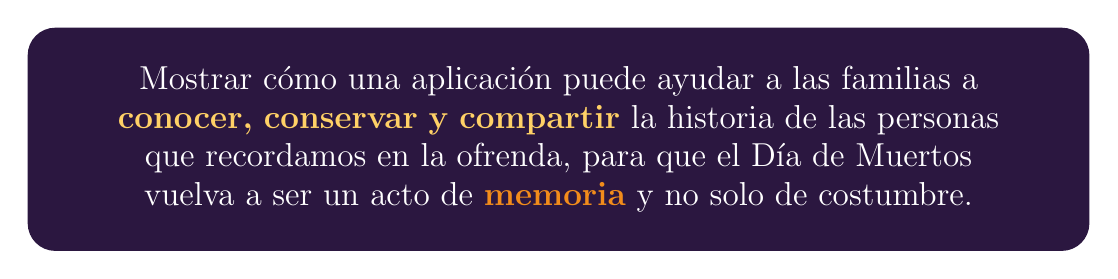
\begin{tikzpicture}
    \node[fill=noche,text=white,rounded corners=10pt,text width=12.5cm,align=center,inner sep=14pt,font=\large] {
      Mostrar cómo una aplicación puede ayudar a las familias a \textbf{\color{vela}conocer, conservar y compartir}
      la historia de las personas que recordamos en la ofrenda, para que el Día de Muertos
      vuelva a ser un acto de \textbf{\color{cempa}memoria} y no solo de costumbre.};
  \end{tikzpicture}
  \end{center}

%  \begin{columns}[T]
%    \column{0.3\textwidth}\centering{\color{rosa}\bfseries\Large 1}\\{\small Entender qué se pierde cuando no conocemos a nuestros difuntos.}
%    \column{0.3\textwidth}\centering{\color{cempa}\bfseries\Large 2}\\{\small Presentar una propuesta para conservar su historia.}
%    \column{0.3\textwidth}\centering{\color{nochesuave}\bfseries\Large 3}\\{\small Reflexionar sobre el valor de recordar.}
 % \end{columns}

\end{frame}

% ---------- Información relevante ----------
\newcommand{\dato}[3]{% color, cifra, texto
  \begin{tikzpicture}[baseline=(current bounding box.north)]
    \node[fill=white,draw=#1,line width=1.2pt,rounded corners=8pt,text width=3.05cm,minimum height=2.7cm,align=center,inner sep=7pt,drop shadow={opacity=0.12}] {%
      {\color{#1}\fontsize{22}{24}\selectfont\bfseries #2}\\[6pt]\footnotesize #3};
  \end{tikzpicture}}
\begin{frame}[plain]
  \papelpicado
  \vspace{0.85cm}
  \begin{center}
    {\fontsize{20}{26}\selectfont\bfseries\color{noche} Una tradición que vive de la memoria}\\[4pt]
%    {\color{gris}\small Se celebra el 1 y 2 de noviembre: la ofrenda recibe a quienes regresan a visitarnos.}
  \end{center}
  \vspace{0.25cm}
  \centering
  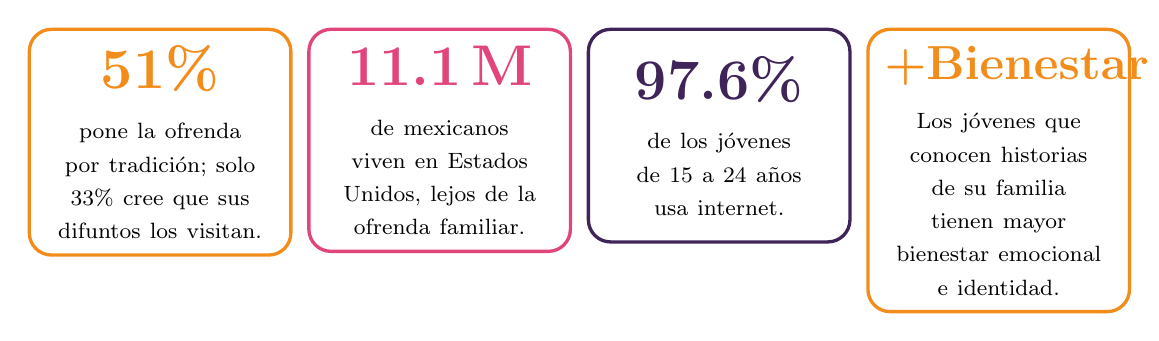
\begin{tikzpicture}
    \node[d=cempa] at (0,0) {{\color{cempa}\fontsize{22}{24}\selectfont\bfseries 51\%}\\[6pt]\footnotesize pone la ofrenda por tradición; solo 33\% cree que sus difuntos los visitan.};
    \node[d=rosa] at (3.55,0) {{\color{rosa}\fontsize{22}{24}\selectfont\bfseries 11.1 M}\\[6pt]\footnotesize de mexicanos viven en Estados Unidos, lejos de la ofrenda familiar.};
    \node[d=nochesuave] at (7.1,0) {{\color{nochesuave}\fontsize{22}{24}\selectfont\bfseries 97.6\%}\\[6pt]\footnotesize de los jóvenes de 15 a 24 años usa internet.};
    \node[d=cempa] at (10.65,0) {{\color{cempa}\fontsize{16}{24}\selectfont\bfseries\mbox{+Bienestar}}\\[6pt]\footnotesize Los jóvenes que conocen historias de su familia tienen mayor bienestar emocional e identidad.};
  \end{tikzpicture}
  \vspace{0.35cm}

  {\color{rosa}\bfseries La tradición ya está en cada casa. Sus historias también pueden estarlo.}\\[5pt]
%  {\tiny\color{gris} Fuentes: encuesta De las Heras (2021); Migration Policy Institute (2024); INEGI, ENDUTIH (2025); Fivush y Duke, Universidad Emory (2010).}
\end{frame}

% ---------- Ejemplo / experiencia ----------
\begin{frame}[plain]
  \papelpicado
  \vfill
  \img{historia}{%
  \begin{columns}[c]
    \column{0.34\textwidth}\centering \polaroid{3.8cm}{4.6cm}{-3}
    \column{0.6\textwidth}\raggedright
    {\color{rosa}\small\bfseries UNA HISTORIA REAL}\\[10pt]
    {\fontsize{19}{25}\selectfont\bfseries\color{noche} “Hablan mucho de él.\\ Pero yo casi no sé quién fue.”}\\[0.6cm]
    {\color{tinta!85} Cada año, en la ofrenda, mi abuelita pone la foto de su papá.
    Yo nunca lo conocí. En la familia hablan mucho de él,
    pero la verdad es que no sé mucho: solo pedacitos que escucho en la sobremesa.}\\[0.5cm]
    {\color{cempa}\bfseries Lo recordamos cada año\ldots{} sin que yo sepa realmente a quién recuerdo.}
  \end{columns}}{%
  \begin{center}
  \begin{minipage}{0.8\textwidth}\centering
    {\color{rosa}\small\bfseries UNA HISTORIA REAL}\\[10pt]
    {\fontsize{22}{28}\selectfont\bfseries\color{noche} “Hablan mucho de él.\\ Pero yo casi no sé quién fue.”}\\[0.6cm]
    {\large\color{tinta!85} Cada año, en la ofrenda, mi abuelita pone la foto de su papá.
    Yo nunca lo conocí. En la familia hablan mucho de él,
    pero la verdad es que no sé mucho: solo pedacitos que escucho en la sobremesa.}\\[0.5cm]
    {\large\color{cempa}\bfseries Lo recordamos cada año\ldots{} sin que yo sepa realmente a quién recuerdo.}
  \end{minipage}
  \end{center}}
  \vfill
\end{frame}

% ---------- Lo que se pierde ----------
\begin{frame}[plain]
  \papelpicado
  \vspace{0.7cm}
  \begin{center}
    {\fontsize{22}{28}\selectfont\bfseries\color{noche} Lo que se pierde cada año}
  \end{center}
  \vspace{0.4cm}
  \centering
  \tarjeta{rosa}{Una foto sin historia}{Conocemos su cara, pero no a qué se dedicaba, qué le gustaba o cómo reía.}\hfill
  \tarjeta{cempa}{Recuerdos que se olvidan}{Las anécdotas se cuentan una vez en la sobremesa y nadie las guarda.}\hfill
  \tarjeta{nochesuave}{Una familia dispersa}{Fotos en cajas, audios en el celular de alguien, primos en otras ciudades.}
\end{frame}

% ---------- 5. Lo que hace ----------
\begin{frame}[plain]
  \papelpicado
  \vspace{0.8cm}
  \begin{center}
    {\fontsize{20}{26}\selectfont\bfseries\color{noche} \color{noche}Ofrenda Viva\\[4pt]{\color{cempa}\large\mdseries Todo lo que fueron, en un solo lugar.}}
  \end{center}
  \begin{columns}[T]
    \column{0.3\textwidth}\centering
      \icono{rosa}{\fill[white,rounded corners=2pt] (-0.45,-0.35) rectangle (0.45,0.4);
                   \fill[rosa] (-0.35,-0.25) rectangle (0.35,0.3);
                   \fill[white] (0,0.08) circle (0.11); \fill[white] (-0.2,-0.25) arc (180:0:0.2);}\\[8pt]
      {\large\bfseries\color{rosa} Su historia}\\[4pt]
      {\small Quién fue, de dónde venía,\\ qué le gustaba.}
    \column{0.3\textwidth}\centering
      \icono{cempa}{\fill[white,rounded corners=4pt] (-0.15,-0.05) rectangle (0.15,0.5);
                    \draw[white,line width=1.6pt] (-0.3,0.15) arc (180:360:0.3); \draw[white,line width=1.6pt] (0,-0.15) -- (0,-0.45);}\\[8pt]
      {\large\bfseries\color{cempa} Su voz}\\[4pt]
      {\small Los recuerdos de la familia,\\ contados por ellos mismos.}
    \column{0.3\textwidth}\centering
      \icono{noche}{\foreach \i in {0,...,3}{\foreach \j in {0,...,3}{
                      \pgfmathtruncatemacro{\q}{mod(\i*5+\j*3+\i*\j,3)}
                      \ifnum\q=0 \fill[white] (-0.4+\i*0.2,0.4-\j*0.2) rectangle ++(0.17,-0.17);\fi}}
                    \draw[vela,line width=1.2pt] (-0.5,0.5) rectangle (0.5,-0.5);}\\[8pt]
      {\large\bfseries\color{noche} Su lugar en la ofrenda}\\[4pt]
      {\small Escanea su foto\\ y conócelo.}
  \end{columns}
\end{frame}



% ---------- Demo en video ----------
\begin{frame}[plain]
  \papelpicado
  \begin{columns}[c]
    \column{0.5\textwidth}
      {\color{rosa}\small\bfseries DEMO}\\[6pt]
      {\fontsize{24}{30}\selectfont\bfseries\color{noche} Así se vive\\ Ofrenda Viva.}\\[0.5cm]
      {\large\color{tinta!85} Conoce a José, escucha a la abuela Carmen y descubre el significado de cada elemento de la ofrenda.}
    \column{0.42\textwidth}
      \centering
      \vspace{0.6cm}
      \iphonevideo{6.1cm}
  \end{columns}
\end{frame}

% ---------- Síntesis ----------
\begin{frame}[plain]
  \papelpicado
  \vspace{0.7cm}
  \begin{center}
    {\fontsize{22}{28}\selectfont\bfseries\color{noche} Lo que nos llevamos}
  \end{center}
  \vspace{0.3cm}
  \centering
  \tarjeta{rosa}{La memoria se pierde}{Ponemos en la ofrenda fotos de personas cuya historia no conocemos.}\hfill
  \tarjeta{cempa}{Puede conservarse}{Ofrenda Viva reúne su historia, su voz y su lugar en la familia.}\hfill
  \tarjeta{nochesuave}{La tradición se fortalece}{Recordar con conocimiento le devuelve el sentido a la ofrenda.}
\end{frame}


% ---------- Reflexión y cierre ----------
{\setbeamercolor{background canvas}{bg=noche}
\begin{frame}[plain]
  \img{cierre}{%
    \begin{tikzpicture}[remember picture,overlay]
      \node[inner sep=0,anchor=center] at (current page.center) {\includegraphics[width=\paperwidth,height=\paperheight]{\imgpath}};
      \fill[noche,opacity=0.82] (current page.south west) rectangle (current page.north east);
    \end{tikzpicture}}{}
  \papelpicado
  \vfill
  \begin{center}
    \begin{minipage}{0.85\textwidth}\centering
      {\color{white}\large Nuestros abuelos guardan historias que ningún libro tiene.\\[3pt]
      Cada año que pasa sin preguntarles, es una historia menos.}\\[1.0cm]
      {\color{cempa}\fontsize{24}{30}\selectfont\bfseries Porque nadie muere del todo\\ mientras alguien lo recuerde.}
    \end{minipage}
  \end{center}
  \vfill
\end{frame}}

% ---------- Gracias ----------
{\setbeamercolor{background canvas}{bg=noche}
\begin{frame}[plain]
  \papelpicado
  \vfill
  \begin{center}
    {\color{white}\fontsize{44}{48}\selectfont\bfseries Gracias}\\[0.4cm]
    {\color{cempa}\Large Ofrenda Viva}\\[1.0cm]
    {\color{white!85}\large Aldo Axel Estrada Zacarías}\\[4pt]
    {\color{white!85}\large Evelin Jiménez Olivo}\\[4pt]
    {\color{white!85}\large Oscar Cabrera Rojas}\\[0.8cm]
    {\color{white!50}\small iOS Development Lab}
  \end{center}
  \vfill
\end{frame}}

\end{document}